\documentclass[a2paper, 8pt,hyperref={implicit=false,draft=false},usenames, dvipsnames]{beamer}
% \usecolortheme{whale}
%\beamertemplateshadingbackground{white!10}{blue!10}
% \usefonttheme[10pt]{professionalfonts} 
% \usefonttheme[10pt]{structuresmallcapsserif} 
\usefonttheme[8pt]{serif}
\usecolortheme{Moris}

% \setbeamercovered{transparent}
\setbeamertemplate{footline}[frame number]
\mode<presentation>
{
% \setbeamertemplate{background canvas}[vertical shading][bottom=red!10,top=blue!10]%
  % \usetheme{Boadilla}
  \usetheme{bjeldbak}
  % \usefonttheme[onlysmall]{structurebold}
}
%\usecolortheme {seahorse}
\setbeamertemplate{caption}{\insertcaption}
\setbeamertemplate{caption label separator}{} %\usetheme{Madrid}
\setbeamertemplate{headline}{}

\usepackage{ulem}
\usepackage[export]{adjustbox}
\usepackage{soul} %for a strike-out font
\usepackage{fontenc}
\usepackage[utf8]{inputenc}
\usepackage{mathtext}
\usepackage{amssymb,amsthm,amsmath}
\usepackage{enumerate}
% \usepackage{hyperref}
\usepackage{graphics}
\usepackage{gensymb}
\usepackage{relsize}
% \usepackage{graphicx}
\usepackage{tcolorbox}
\usepackage{tikz} %for flowcharts
\usetikzlibrary{positioning, fit, shapes}
\beamertemplatenavigationsymbolsempty
\setbeamertemplate{footline}[frame number]

\AtBeginSection[]
{%
}

% \definecolor{MashaBlue}{HTML}{003E6D}
% \definecolor{DeepBlue}{RGB}{35,80,120}
% \definecolor{AccentBlue}{RGB}{20,130,165}
% \definecolor{AccentGreen}{RGB}{200,225,200}

% \setminted{linenos=true}
\newcommand{\minbul}{\item[$\textcolor{Turquoise}{\bullet}$]}
% \newcommand{\minbul}{\item[$\textcolor{Dandelion}{\bullet}$]}
\newcommand{\bul}{\item[$\textcolor{BurntOrange}{\bullet}$]}
\newcommand{\warnbul}{\item[$\textcolor{BrickRed}{\bullet}$]}
\newcommand{\extrabul}{\item[$\textcolor{OliveGreen}{\bullet}$]}
% \newcommand{\minbul}{\item[$\textcolor{Bittersweet}{\bullet}$]}
\newcommand{\NavyBlue}{\textcolor{NavyBlue}}
\newcommand{\BrickRed}{\textcolor{BrickRed}}
\newcommand{\blue}{\textcolor{blue}}
\newcommand{\red}{\textcolor{red}}
\newcommand{\cyan}{\textcolor{cyan}} 
\newcommand{\Carbon}{$^{14}\text{C}$}
\newcommand{\Losc}{\ensuremath{L^{\text{osc}}}}
\newcommand{\Lcoh}{\ensuremath{L^{\text{coh}}}}
\newcommand{\Ld}{\ensuremath{L^{\text{d}}}}
\newcommand{\Dm}{\ensuremath{\Delta m^2}}
\newcommand{\Important}{\textcolor{BrickRed}}
\newcommand{\Regular}{\textcolor{DeepBlue}}
\newcommand{\MashaBlue}{\textcolor{MashaBlue}}
\newcommand{\MidnightBlue}{\textcolor{MidnightBlue}}
\newcommand{\Orange}{\textcolor{Orange}}
\newcommand{\Maroon}{\textcolor{Maroon}}
\newcommand{\Bittersweet}{\textcolor{Bittersweet}}
\newcommand{\regitem}{\item[\Regular{$\bullet$}]}
\newcommand{\impitem}{\item[\Important{$\bullet$}]}
\newcommand{\midblitem}{\item[\MidnightBlue{$\bullet$}]}
\newcommand{\orangeitem}{\item[\Orange{$\bullet$}]}
\newcommand{\pineitem}{\item[\Maroon{$\bullet$}]}
\newcommand{\bitteritem}{\item[\Bittersweet{$\bullet$}]}
\newcommand{\sip}{\ensuremath{\sigma_p}}
\newcommand{\srel}{\ensuremath{\sigma_{\text{rel}}}}
\newcommand{\six}{\ensuremath{\sigma_x}}
\newcommand{\anue}{\ensuremath{\bar{\nu}_e}}

\setbeamertemplate{logo}{
  
\includegraphics[scale=0.2]{../pics/logo_dyb.png}
  
\includegraphics[scale=0.3]{../pics/JINR_logo.png}
}

\begin{document}
  \institute[JINR]{\large{Joint Institute for Nuclear Research, Russia}}
  \title{\BrickRed{Experimental study of decoherence effects in neutrino
    oscillations in Daya Bay}}
    \author{\BrickRed{Konstantin Treskov} on behalf of Daya Bay
    collaboration}
    \date{\MashaBlue{Monday session, Poster Wall \MashaBlue{\#160}}}

  \logo
  
  
  % \titlegraphic{\includegraphics[scale=0.08]{./pics/DLNP_2_tr.png}}
  % \titlegraphic{
\includegraphics[scale=0.08]{./pics/JINR_logo.png}}
\begin{frame}
\titlepage
\end{frame}

\small
\begin{frame}
\begin{itemize}
    \item Treatment of flavor states as a \Regular{superposition of mass states
        with different momenta}, \Important{wave packets}, resolves
        inconsistencies of plane wave approach and leads to \Important{new
        effects} (Gaussian form factor for wave packet is assumed):
        \begin{itemize}
            \item \MidnightBlue{Loss of coherence} due to \MidnightBlue{different group
                    velocities of wave packets} and \Orange{spacial localization of
                production/detection regions}.
            \item \Important{Partial restoration of coherence} due to wave
                packet spacial broadening.
        \end{itemize}
          \colorbox{CornflowerBlue!15}{\raisebox{0}[1.1\height]{\makebox[34em]{
        \begin{equation*}
         P_{\alpha\beta}(L) = \sum \limits_{k,\,j=1}^3\frac{ V^{\phantom\dagger}_{k
                 \beta }V^*_{\alpha k}V^{\phantom\dagger}_{j \alpha }
                 V^*_{\beta j} }{\Maroon{\sqrt[4]{1 +
             \left(L/\Ld_{kj}\right)^2}}}\,\,
             \exp{\left[-\frac{\textcolor{MidnightBlue}{\left(L/\Lcoh_{kj}\right)^2}}{\Maroon{1+\left(L/\Ld_{kj}\right)^2}}
    -\textcolor{Orange}{\mathrm{D}^2_{kj}\right]}}
    \text{e}^{-i(\varphi_{kj} + \varphi^d_{kj})}
    \end{equation*}
     }}}
 \item \Regular{Multiple reactor-detector baselines allow to constrain}
     relative  momentum dispersion of wave packets
     \Important{\srel} in Daya Bay.
\end{itemize}
\begin{columns}[T]
   \begin{column}{0.5\textwidth}
       \setbeamercolor{itemize item}{fg=OliveGreen!70}
       \begin{itemize}
           \item \Important{8} detectors and \Important{6} reactors.
           \item \anue\, detection through inverse beta-decay 
               {\hspace*{1.3cm}\centering{\Important{$\anue + p \rightarrow e^+ + n$}}}
            \item Use coincidence of prompt and delayed signals in time to select
                \anue\, events.
           \item Rich event sample \Important{\ensuremath{\anue \sim 10^6}}:
                    {\centering
                    \begin{table*}
                        \renewcommand{\arraystretch}{1.2}
                        \begin{tabular}{@{}cccc{}@}
                            \toprule
                        & \Regular{EH1} & \Regular{EH2} & \Regular{EH3}\\
                            \Regular{Events}\,\,\, & \Important{613813}\, &
                            \Important{477144}\, & \Important{150255}
                            \bottomrule
                        \end{tabular}
                    \end{table*}}
                    \vskip1ex
           \item Energy resolution \ensuremath{\sim 8\,\%} at 1~MeV.
       \end{itemize}    
    \end{column}
    \begin{column}{0.5\textwidth}
        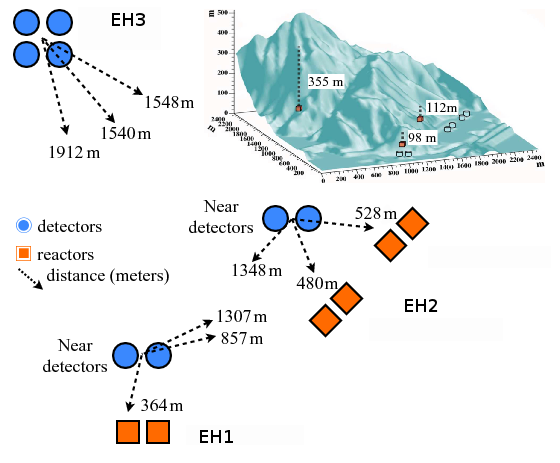
\includegraphics[scale=0.25]{../pics/DYBdiag_3.png}
    \end{column}
\end{columns}
\end{frame}

\begin{frame}
    \begin{columns}[T]
        \begin{column}{0.55\textwidth}
            \begin{itemize}
            \item Statistical analysis based on \Important{fixed-level
                \ensuremath{\Delta \chi^2}} (systematics propagated wih
                covariance matrix) and \Important{Feldman-Cousins} approach with free
                \Important{\srel}, \Important{\ensuremath{\sin^2
                2\theta_{13}}}, \Important{\ensuremath{\Dm_{32}}}, flux normalization \Important{N}
            shows 3 distinct regions:
                \begin{itemize}
                    \item \Important{$\srel < 10^{-16}$} -- oscillations are suppressed
                        by \ensuremath{\text{D}^2} (spacial size of reactor
                        cores).
                    \item \Important{$10^{-16} < \srel < 0.1$} -- no impact on
                    oscillations.
                    \item \Important{$\srel > 0.1$} -- loss of coherence
                    due to spacial separation
                    \Important{\Lcoh} and dispersion \Important{\Ld}.
                \end{itemize}
            % \item First experimental limits on spacial size of wave packet are:
                % \begin{center}
                    % \colorbox{OliveGreen!20}{\raisebox{0}[1.2\height]{\makebox[13em][c]{
                    % \begin{equation*}
                        % 10^{-11}\, \text{cm} \lesssim \six \lesssim 2\, \text{m}
                    % \end{equation*}
                    % }}}
                % \end{center}
        \end{itemize}
        \begin{columns}
            \begin{column}{0.5\textwidth}
                \centering
                \begin{figure}
                    \vspace*{-0.5cm}
                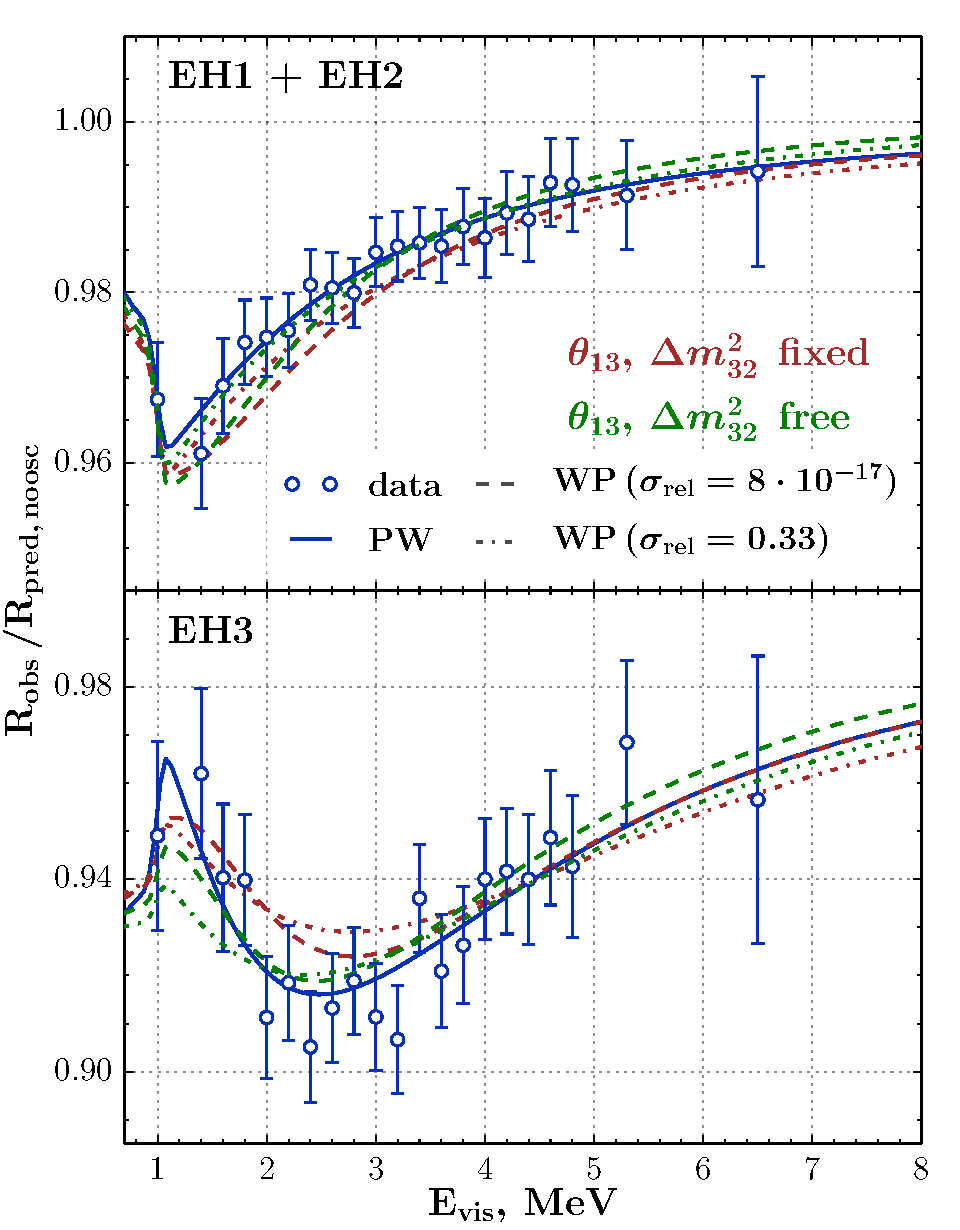
\includegraphics[scale=0.23]{../pics/EH-ratio_5sigma-s_double-EH_bold.pdf}
                \end{figure}
            \end{column}
            \begin{column}{0.5\textwidth}
                \vspace*{-0.6cm}
                \begin{itemize}
                    \item \Important{Allowed region} for \Important{\srel}\, at 95\%~C.L.:
                \begin{center}
                    \vspace*{-0.2cm}\hspace*{-0.5cm}\colorbox{OliveGreen!20}{\raisebox{0}[1.2\height]{\makebox[13em][c]{
                    \begin{equation*}
                        \hspace*{-0.12cm}2.38 \cdot 10^{-17} < \srel < 0.232
                    \end{equation*}
                    }}}
                \end{center}
                    \item \Important{First experimental limits} on spacial size of wave packet are:
                    \begin{center}
                        \vspace*{-0.2cm}\hspace*{-0.5cm}\colorbox{OliveGreen!20}{\raisebox{0}[1.2\height]{\makebox[12em][c]{
                        \begin{equation*}
                            10^{-11}\, \text{cm} \lesssim \six \lesssim 2\, \text{m}
                        \end{equation*}
                        }}}
                    \end{center}
                \item Upper limit on \Important{\srel{}} is:
                \begin{center}
                    \vspace*{-0.2cm}\hspace*{-0.5cm} \colorbox{OliveGreen!20}{\raisebox{0}[1.2\height]{\makebox[12em]{\ensuremath{\srel{}
                    < 0.2} at 95\% C.L.}}}
                \end{center}
                % \item The \Important{insignificance} of decoherence effect ensure
                    % \Important{unbiased measurent} of oscillation parameters in Daya Bay.
                \end{itemize}
            \end{column}
        \end{columns}
            % \centering
            % \begin{figure}
                % \vspace*{-0.5cm}
            % 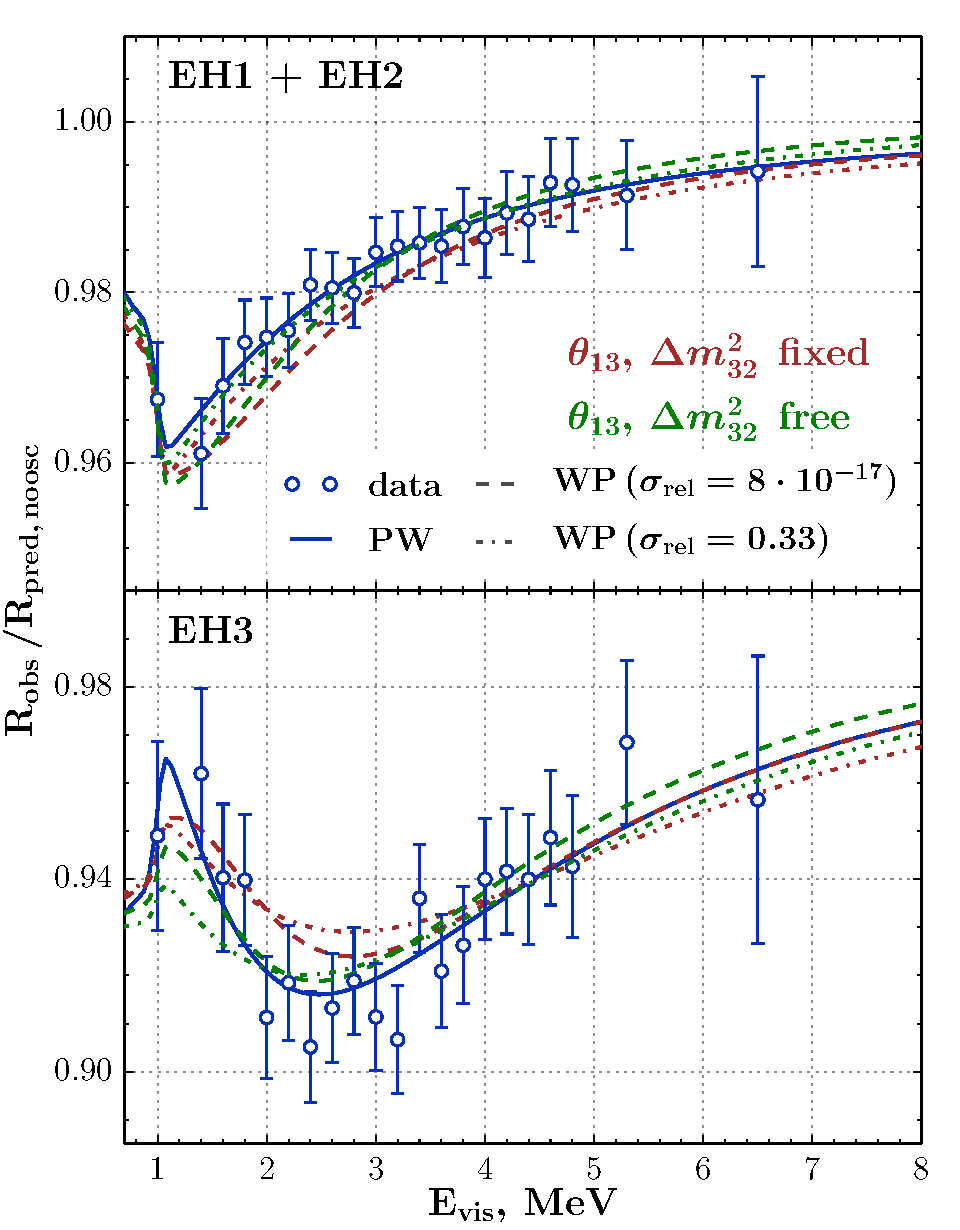
\includegraphics[scale=0.22]{../pics/EH-ratio_5sigma-s_double-EH_bold.pdf}
            % \end{figure}
        \end{column}
        \begin{column}{0.5\textwidth}
            \begin{figure}
            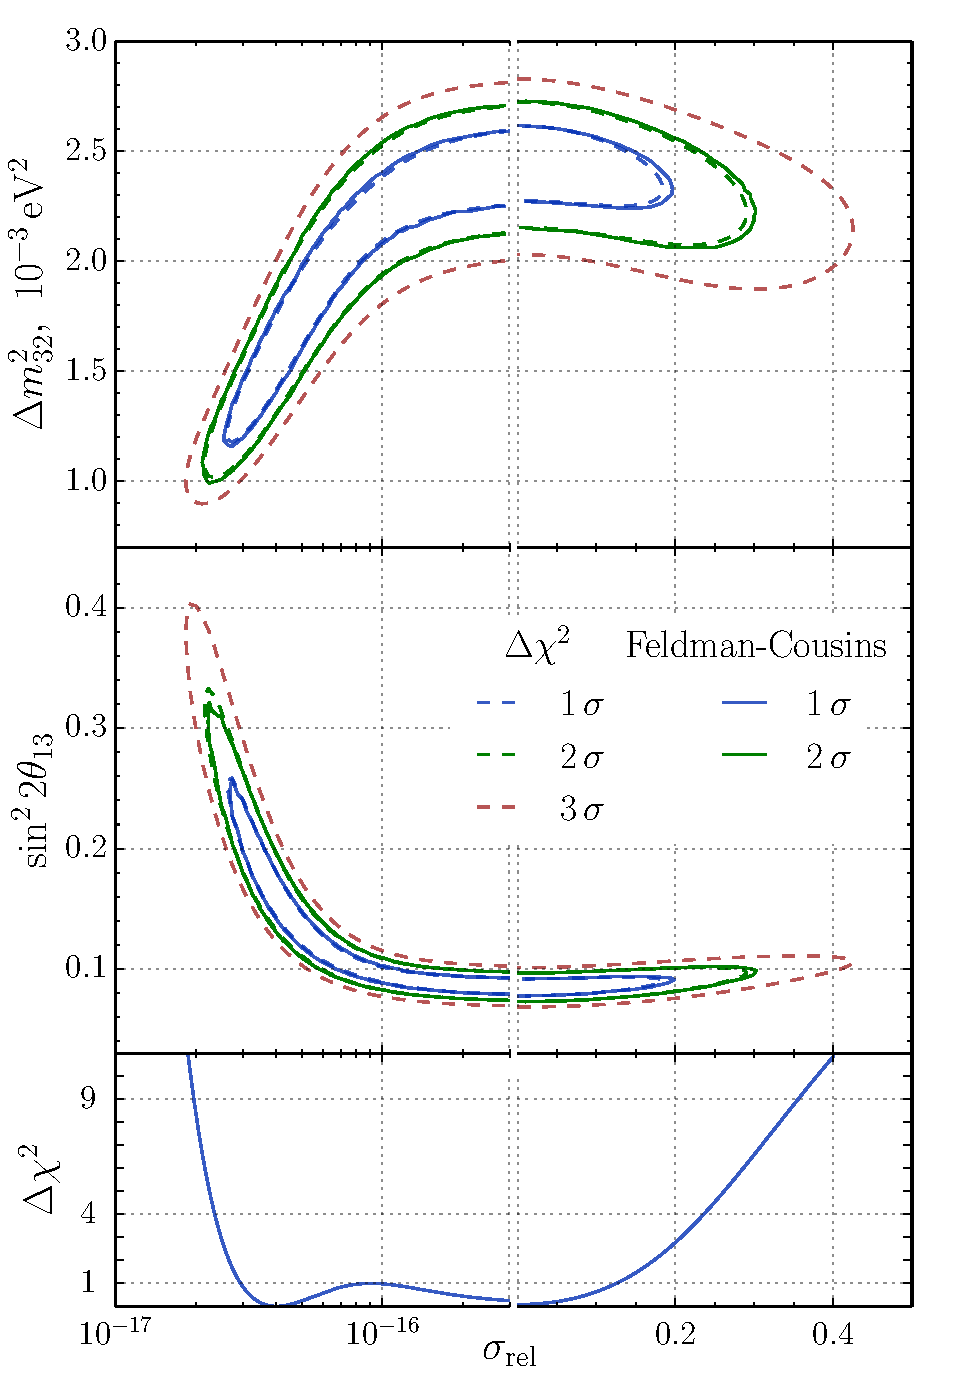
\includegraphics[scale=0.3]{../pics/scan_db_s-dm-th_ihep-fc_v2.pdf}
            \end{figure}
            \begin{itemize}
                % \item The upper limit on \Important{\srel{}} is:
                % \begin{center}
                    % \colorbox{OliveGreen!20}{\raisebox{0}[1.2\height]{\makebox[13em]{\ensuremath{\srel{}
                    % < 0.2} at 95\% C.L.}}}
                % \end{center}
            \item The \Important{insignificance} of decoherence effect ensures
                \Important{unbiased measurent} of oscillation parameters in Daya Bay.
            \end{itemize}
        \end{column}
    \end{columns}
\end{frame}

\end{document}
